

\subsection{Graphical Representation}
\bigskip

\subsubsection{UI State Diagrams}
\medskip
The graphical user interface will be designed for two distinct users interacting with the system. The first is primary user, the emergency first responder. This user will only need access to the map view and system status overview, their user interaction state diagram is shown below.

\medskip
\begin{figure}[H]
\centering
    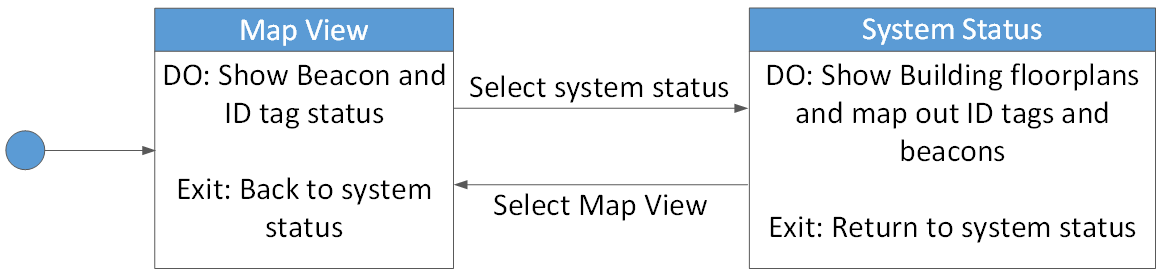
\includegraphics[scale=0.4]{./images/UI_State_FF.png}
    \caption{UI State Diagram - Primary User}
    \label{UISD-1}
\end{figure}
\medskip

The secondary user will be the administrator of the system. For secondary users the interaction is much more complex and require a more in depth level of user interaction. The secondary user interaction state diagram is shown below.

\medskip
\begin{figure}[H]
\centering
    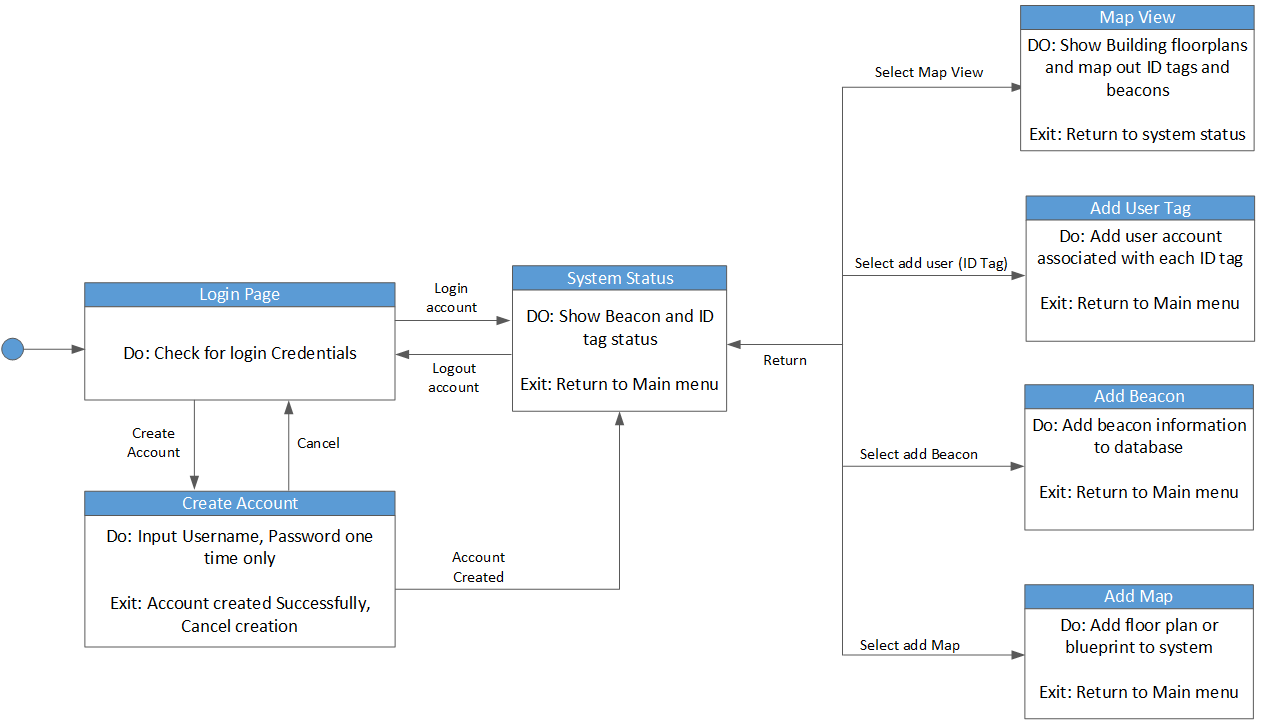
\includegraphics[scale=0.5]{./images/UI_State_IT.png}
    \caption{UI State Diagram - Secondary User}
    \label{UISD-2}
\end{figure}
\medskip



\pagebreak
\subsubsection{UI Mock-Ups}
\medskip
In the Proof of concept a simple console output displaying only the basic information such as the MAC address, RSSI and distance calculations between each beacon and id tag would be shown. Similar to the figure presented below. This UI is just to demonstrate the feasibility of the initial beacon systems.

\medskip
\begin{figure}[H]
\centering
    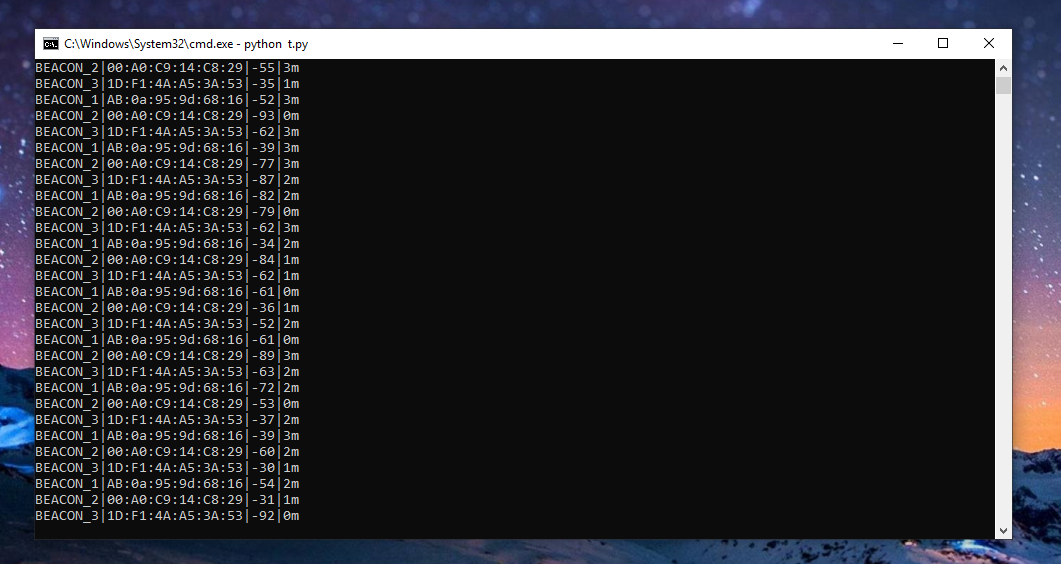
\includegraphics[scale=0.5]{./images/UI_PoC.png}
    \caption{PoC Console UI}
    \label{UI_PoC}
\end{figure}
\medskip

In the prototype phase of development, the user interface would resemble a wireframe of the final implementation. A simple box map is used to display user location in near real time similar to the figure below.

\medskip
\begin{figure}[H]
\centering
    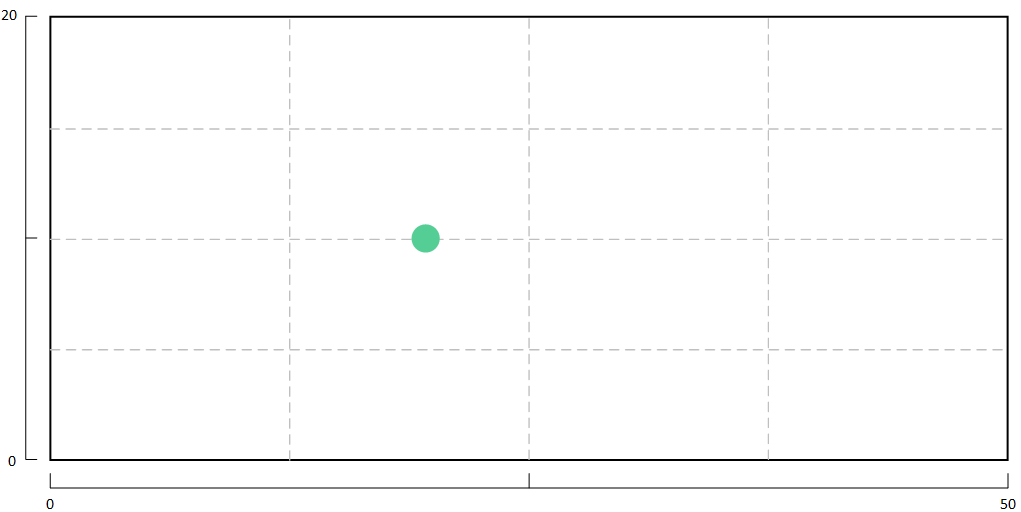
\includegraphics[scale=0.6]{./images/UI_box.png}
    \caption{Prototype Box Map Layout View}
    \label{UI_box}
\end{figure}

\pagebreak

In the Final phase of development the user interface would be complete, resulting in a UI that would fulfil the necessary needs of all users of the system. The primary user would have access to the map view and the system status view shown in figure \ref{map_ff} and \ref{ss_ff}.

\medskip
\begin{figure}[H]
\centering
    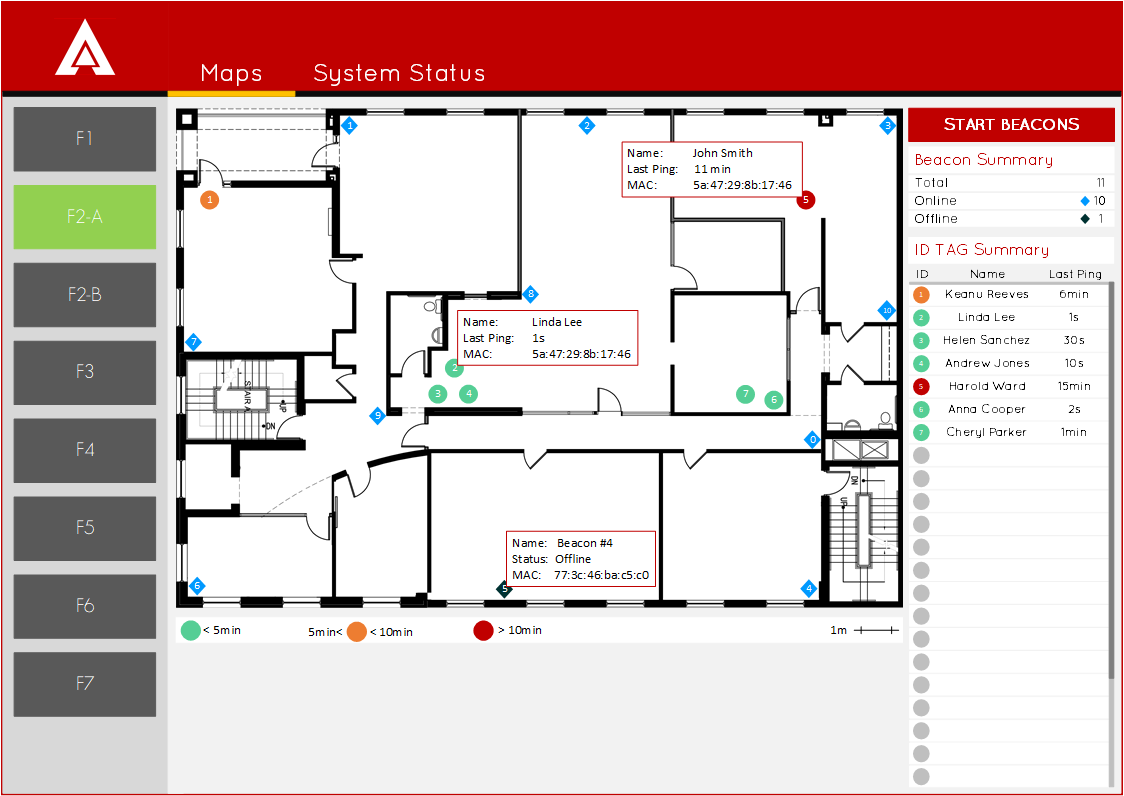
\includegraphics[scale=0.45]{./images/UIMU_map_ff.png}
    \caption{Primary User Map View}
    \label{map_ff}
\end{figure}

\begin{figure}[H]
\centering
    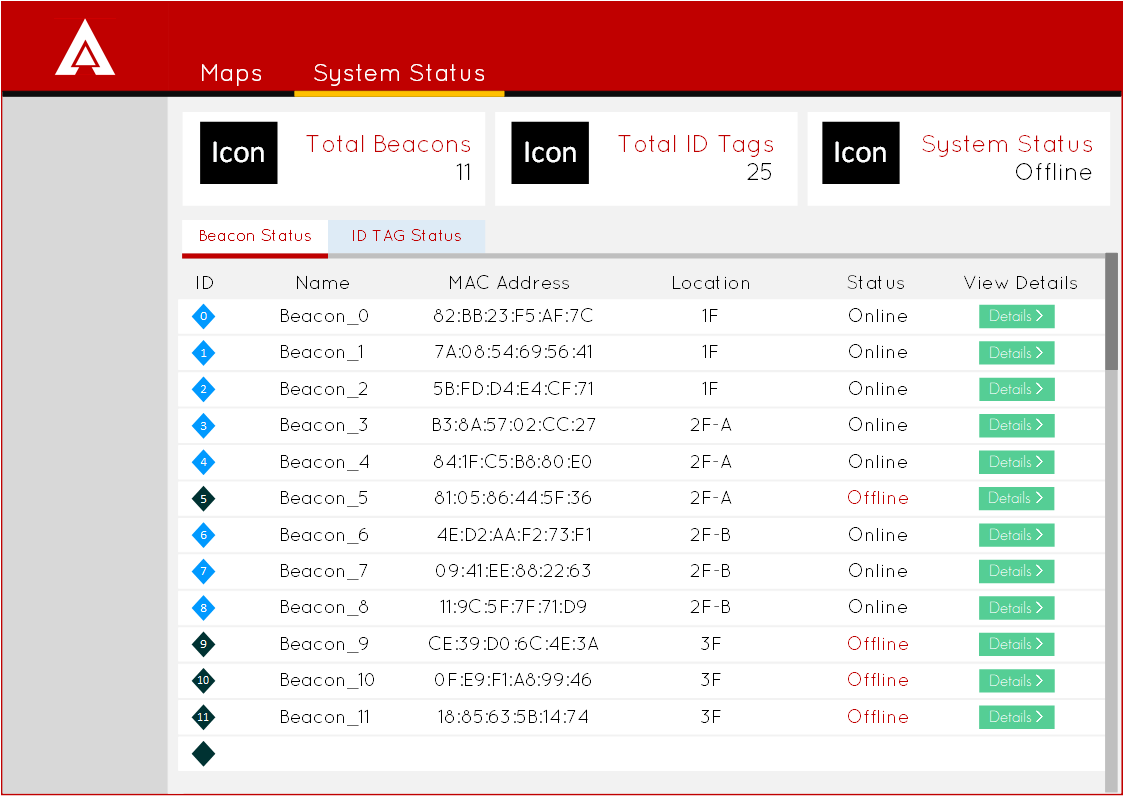
\includegraphics[scale=0.45]{./images/UIMU_status_ff.png}
    \caption{Primary User System Status View}
    \label{ss_ff}
\end{figure}
\medskip

\pagebreak
The secondary user, the system administrator will be interacting with the system configurations. The administrator will be performing tasks such as adding/edit beacons, users, and maps or floor plans. The GUI for secondary users are shown in the below figures.

\medskip
\begin{figure}[H]
\centering
    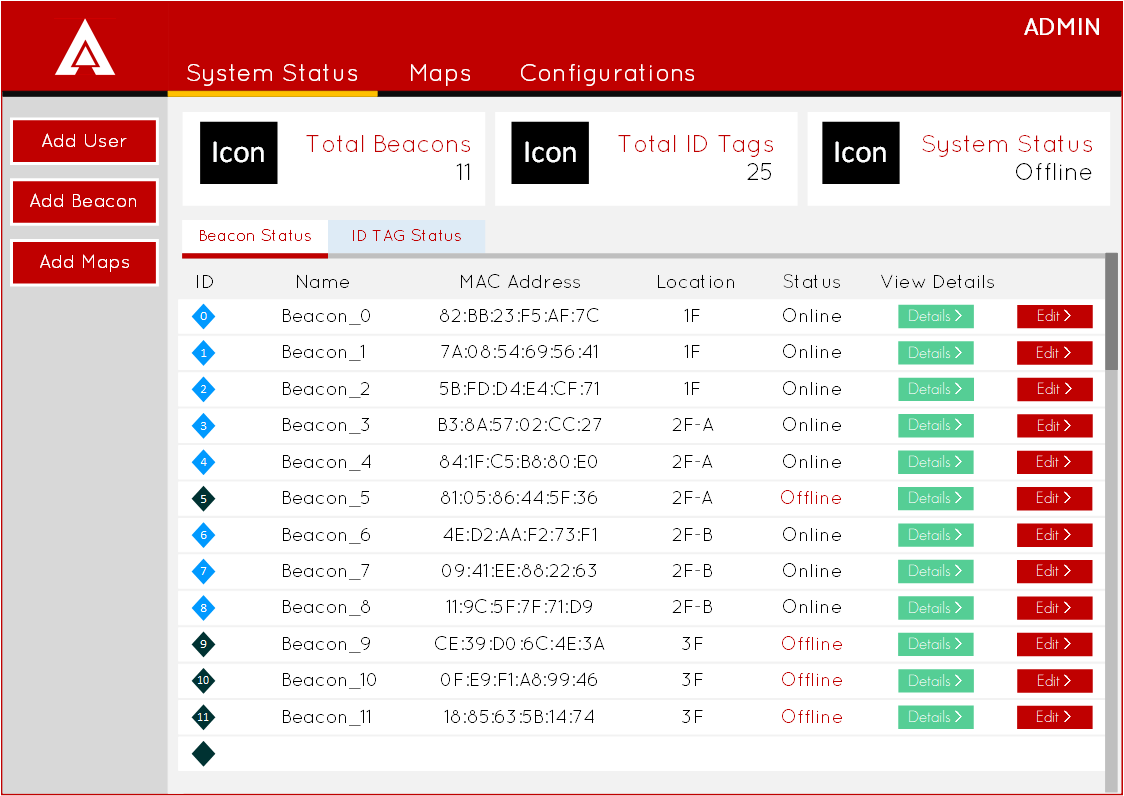
\includegraphics[scale=0.45]{./images/UIMU_status_IT.png}
    \caption{Secondary User System Status View}
    \label{ss_it}
\end{figure}

\medskip
\begin{figure}[H]
\centering
    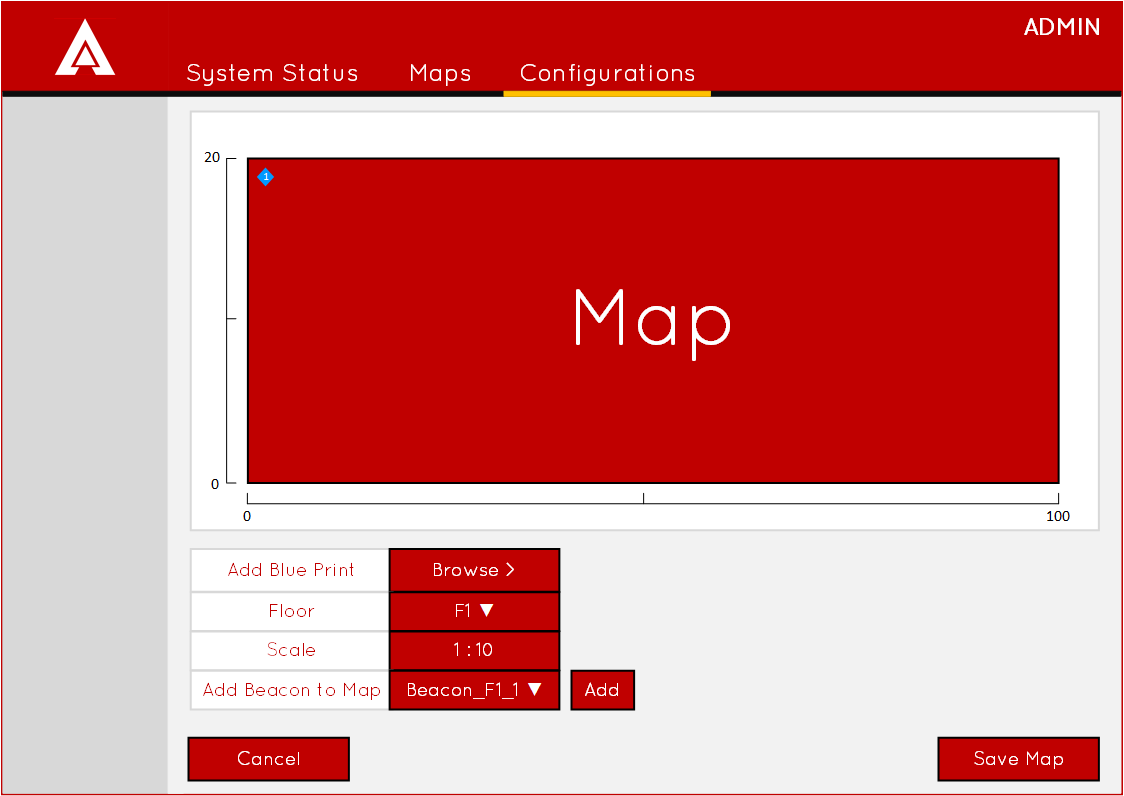
\includegraphics[scale=0.45]{./images/UIMU_add_map.png}
    \caption{Add Map View}
    \label{add_map}
\end{figure}
\pagebreak


\medskip
\begin{figure}[H]
\centering
    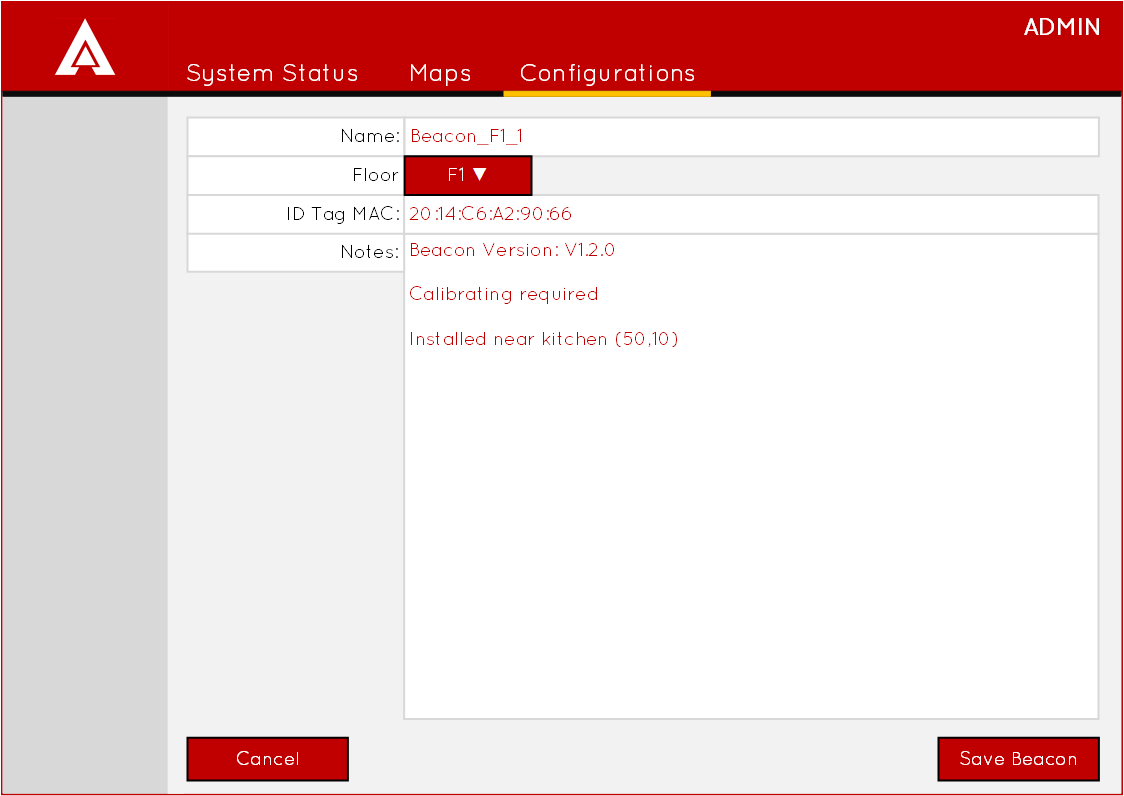
\includegraphics[scale=0.45]{./images/UIMU_add_beacon.png}
    \caption{Add Beacon View}
    \label{add_b}
\end{figure}

\medskip
\begin{figure}[H]
\centering
    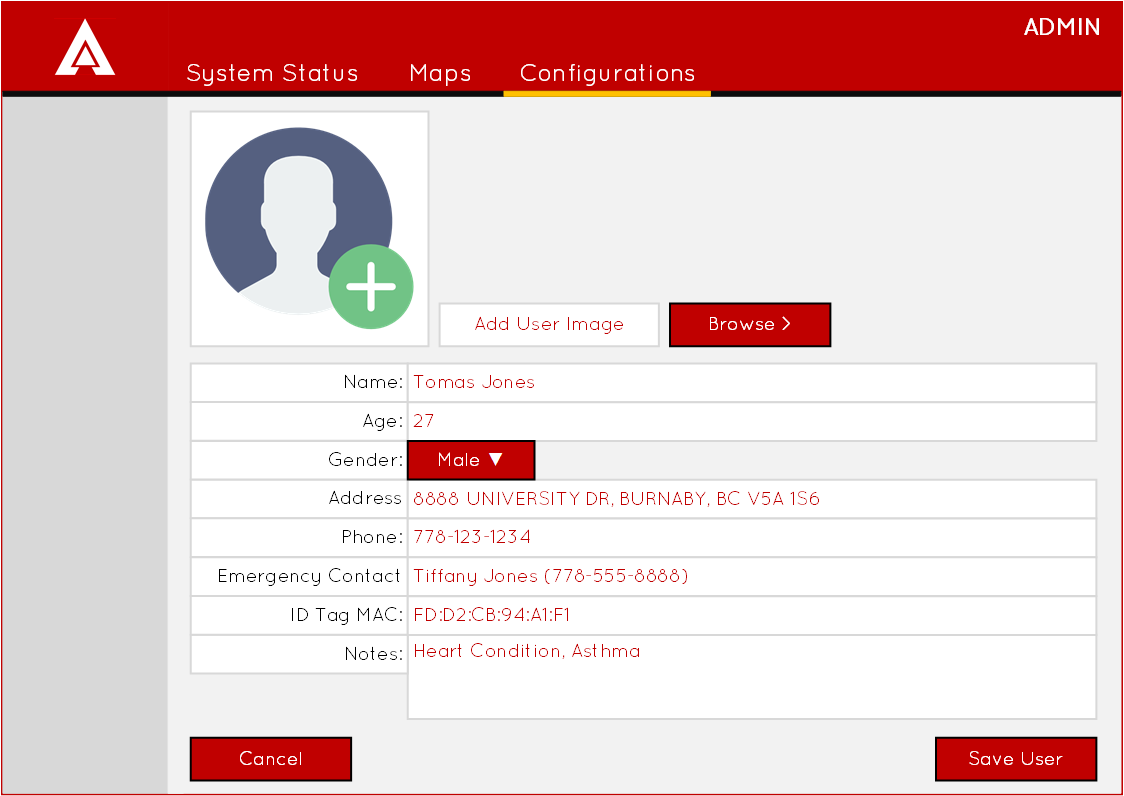
\includegraphics[scale=0.45]{./images/UIMU_add_user.png}
    \caption{Add User View}
    \label{add_user}
\end{figure}





